% This is samplepaper.tex, a sample chapter demonstrating the
% LLNCS macro package for Springer Computer Science proceedings;
% Version 2.20 of 2017/10/04
%
\documentclass[runningheads]{llncs}
%
\usepackage{graphicx}
% Used for displaying a sample figure. If possible, figure files should
% be included in EPS format.
%
% If you use the hyperref package, please uncomment the following line
% to display URLs in blue roman font according to Springer's eBook style:
% \renewcommand\UrlFont{\color{blue}\rmfamily}

\begin{document}
%
\title{Speech Enhancement for Low Quality Audio}
%
%\titlerunning{Abbreviated paper title}
% If the paper title is too long for the running head, you can set
% an abbreviated paper title here
%
\author{Rincewind\inst{1}\orcidID{0000-0000-0000-0000}
\and Luggage\inst{1}\orcidID{0000-0000-0000-0001}}
%
\authorrunning{Rincewind \and Luggage}
% First names are abbreviated in the running head.
% If there are more than two authors, 'et al.' is used.
%
\institute{Unseen University,\\
Ankh-Morpork,\\
The Discworld\\
\email{\{rincewind,luggage\}@unseen-university.ankh-morpork.discworld}}
%
\maketitle              % typeset the header of the contribution
%
\begin{abstract}
The paper presents an attempt to solve the problem of bad audio quality
affecting the listening experience and accuracy of speech-to-text systems. We
describe two experiments: one with automated spectral subtraction and one
with Gycle-GAN domain transfer from the defect to the
pure as a way to reduce the impact of noise, overdrive, reverberation and other
defects.
\keywords{speech recognition, GycleGAN, domain transfer, signal processing}
\end{abstract}

\section{Introduction}

Automatic speech recognition is generally approached by means of machine
learning: a statistical model is inferred based on some training data. Its
application is based on the assumption that whatever was learned about the training
data will also apply to the input data. It is clear then, that if the input
data have different properties than the training data, the basic assumption is
violated and the inference performance will suffer.
Also, if the training data themselves are damaged in a way that makes the desired
information harder to extract, the learning is going to be less successful.

For speech recognition, the problem of noise, reverberation and other defects
has been a pain point and also a point of research. To mention some, Gillespie
and Atlas\cite{gillespie2002diversity} deal with reverberation for
GMM-based ASR, Yoshioka et al.\cite{reverbmagazine} summarize various
dereverberation techniques, Ko et al.\cite{reverbaugment} attempt to
simlulate reverberation in training data digitally. Seltzer, Yu and
Wang\cite{dnnnoiserobust} deal with noise in DNN-based ASR.

There are in principle two ways to deal with the negative effect of acoustic
deficiencies in speech recognition: 1) to adapt the model, which includes
training on augmented data, and 2) to adapt the input data. This article
presents one experiment in the former and one in the latter approach.

\section{Spoken Corpus of Karel Makoň}

We are looking into the problem of acoustic inconsistencies in terms of varying
overall quality, reverberation, noise, overdrive and other phenomena in a
dataset that is to be automatically transcribed and listened to by humans.

The application is at the spoken corpus of Karel Makoň\cite{makondata}, for which
a speech recognition system has been developed\cite{kruuza2012making} but where
the heterogenous acoustic quality affects both the speech recognition
performance and the listening experience. Whereas the word error rate on the
overall test set is 19\%, it is 45\% on a sample of recordings suffering from
overdrive, and 68\% on recordings taken on a magnetophone tape with a slow
recording speed of 2 centimeters per second after some 30 years of living-room
storage.

We are conducting an experiment to make the input data similar to the training
data instead of the more usual other way around because 1) it is not easy to
make the volunteer annotators transcribe acoustically flawed data, 2) not only
speech recognition would benefit from successful denoising, the listening
experience would improve too, and 3) the model could stay leaner.

What acoustic defects are actually present? Since the corpus was digitized from
magnetophone tapes of spontaneous talks of a single speaker recorded in various
amateur conditions and with consumer devices, we can broadly distinguist these
types of quality degradation:
\begin{enumerate}
\item{additive noise -- hum or hiss,}
\item{
    stationary interference like screeching added by low-quality magnetophone
    parts or the erasing head signal,
}
\item{non-stationary interference like background speech or door slams,}
\item{
    room echo or ill-equalized microphone boosting or cutting certain
    frequencies,
}
\item{non-linear distortion of the magnetophone}
\item{speed fluctuations.}
\end{enumerate}

The individual interference types affect each other and can occur several times
in several stages. For instance, the echo is essentially convolution with a certain vector of
amplitude values, known as the impulse response. It might even not be
constant if there are moving objects in the room or if the speaker or
microphone is moving. This convolution is followed by a non-linear
distortion in the microphone and its preamplifier and convolved again with
another impulse response, this time representing a frequency and phase
response of recorder's amplifiers. Finally it is non-linearly distorted in
the process of making a magnetic recording on the tape. Another batch of
distortions comes during the playback. On top of that, in every step a certain
amount of additive noise is introduced. Clearly, modeling, let alone reverting these
interferences is a difficult task.

\section{Denoising}

We conducted a baseline experiment employing the standard denoising based on
spectral subtraction. We assumed that each recording in the
corpus suffers from a consistent kind of noise. This does not hold for all the
recordings but we dismissed this fact for the sake of simplicity. We used sox
fox the denoising routine. The process for each recording is as follows:
\begin{enumerate}
\item{Identify and isolate a sample of pure stationary noise,}
\item{extract the noise profile,}
\item{apply noise reduction based on the noise profile.}
\end{enumerate}

Items 2 and 3 are taken care of by sox. As for extracting fitting silences, we
used the following method:
\begin{enumerate}
\item{
    Identify and extract all precicted silences using an
    existing aligned automatic transcript.
}
\item{
    Select 100 silences around the 25th percentile ordered by length.
    This secures silences that are neither too short nor too long. Long silences
    tend to contain non-stationary noises, that's why we avoid using them.
}
\item{
    Create a distance matrix on the silences using
    musly\cite{schnitzer2011using}.
}
\item{
    Select 10 silences with the lowest median on the distance matrix. These
    silences are most like other silences, thus being least likely to contain
    non-speech events.
}
\item{
    Finally, catenate and output the selected silences.
}
\end{enumerate}

Subjective evaluation confirms the expectable outcome that relatively
high-quality recordings that only suffer from some additive noise get
easier to listen to. Recordings suffering from other defects and overall lower
audio quality sometimes get rather harder to understand.

We have also trained a speech recognition system on the denoised data. The
performance has sunken to word error rate of 0.94, which basically means the
transcription doesn't work at all. Probably with some parameter tweaking this
could be remedied but it doesn't seem to be a promising path. Curiously enough, the
original model trained on non-denoised data performs much better on the denoised
test data with word error rate of 0.70. Table~\ref{tab:results-denoise} sums
these up.

\begin{table}[htpb]
\begin{center}
\begin{tabular}{|l||r|r|}
\hline
WER    & original model & denoised model \\
\hline
original testing data & 0.189 & 0.940 \\
denoised testing data & 0.698 & 0.941 \\
\hline
\end{tabular}
\caption{Word error rate for the original and denoised test data by a model trained
on the original and denoised training data.}\label{tab:results-denoise}
\end{center}
\end{table}

\section{Neural Domain Transfer}

The revolutionary article of Zhu et al.\cite{cyclegan} presenting
cycle-consistent generative adversarial networks gave mankind a mighty tool and
a hilarious toy that was used for de-hazing
photographs\cite{Engin_2018_CVPR_Workshops}, giving people other's facial
expressions\cite{jin2017faceoff}, in biomedicine\cite{yang2018biogan} and also
in speech processing: Kaneko and Tameoka\cite{kaneko2017parallel} present
speech domain transfer and Hosseini-Asl et al.\cite{hosseini2018malevoicegan} do
the same for the purpose of speech recognition.


Most closely related to the work presented in this article is probably
SEGAN\cite{pascual2017segan}: CycleGAN employed to enhance speech.

CycleGAN assumes two datasets in consistent domains: day and night photos,
schematic and photographic maps, male and female speech etc. In this case,
we have a clear consistent domain of clean, high-quality recordings and the
rest, which suffers from any combination of a number of defects. The damaged
recordings are very unlike each other, they don't form a consistent domain.

There are two ways of dealing with this situation: 1) adapt CycleGAN so that it
can deal with a ``compact'' and a ``scattered'' domain or 2) cluster the
data and apply CycleGAN on the individual clusters. While adapting CycleGAN may be a
point of future work, we have explored the simpler way of clustering the data.

\section{Clustering}

In order to perform clustering on any dataset, a metric on the data is needed.
We have used that proposed by Mandel \& Ellis\cite{mandel2005song}, which
is based on mel-frequency cepstra. A distance matrix has been created using
musly and the clusters on top of that using
hierarchical clustering\cite{johnson1967hierarchical}.

A manual... or rather aureal check on the clusters confirms that files falling
into a cluster are indeed acoustically similar. So we arrived at a cluster of
overdriven recordings, a cluster of heavily hummed ones etc.

For curiosity, we looked at the distances of the files among each other and
compared it to that between other familiar sounds. For instance, two adjacent
segments of the same speaker from a meeting of the Czech parliament has a
distance of 1.4. Different speakers have a distance of 6.5. One of these
segments compared to a black metal song chorus has the distance of 519. On the
other hand, the median distance among the Spoken corpus of Karel Makoň, where
there is a single speaker, amounts to 55.9.

The experiment presented below is conducted on three clusters:
\begin{enumerate}
\item{A cluster of the cleanest recordings, used as the destination domain,}
\item{a cluster of overdriven recordings and}
\item{a cluster of recordings taken with low tape speed.}
\end{enumerate}
Recordings in cluster 3 are the hardest to understand even for humans. All these
clusters have a maximum internal distance of 25.

\section{Results}

We have used the voice transfer method as proposed by Kaneko \&
Kameoka\cite{kaneko2017parallel} and implemented by
Mao\footnote{github.com/leimao/Voice\_Converter\_CycleGAN}. We have trained
transfer 1) between the clean and the overdriven cluster and 2) between the
clean and the low-speed cluster.

After 200 epochs, we have performed speech recognition on the transferred data.
The result is summed up in Table~\ref{tab:results}.

\begin{table}[htpb]
\begin{center}
\begin{tabular}{|l||r|r|}
\hline
           & original & transferred \\
\hline
overdriven & 0.450 & 0.441 \\
low-speed  & 0.685 & 0.939 \\
\hline
\end{tabular}
\caption{Word error rate for the two damaged clusters before and after CycleGAN
transfer.}\label{tab:results}
\end{center}
\end{table}

The word error rate decrease in the overdriven cluster is unfortunately statistically
insignificant with standard deviations 0.054 and 0.079 of the transferred and
original versions respectively. An important benefit is
that the transferred overdriven (or should we say de-overdriven) sound files are
much easier on the ear and it can be a help for human listeners.

The wrecking word error rate increase from 69\% to 94\% in case of the
recordings taken at low tape speed requires further investigation.
Figure~\ref{fig:plzen} shows the waveform and spectrum of a sample from the low-speed
cluster before and after the transfer. For comparison,
Figure~\ref{fig:overdrive} shows the same for the overdriven cluster.
Notice how parts of the signal are completely missing in the converted low-speed
sample. It seems that when the signal is too hard to separate from the noise,
the convertor prefers to generate silence.

\begin{figure}[htpb]
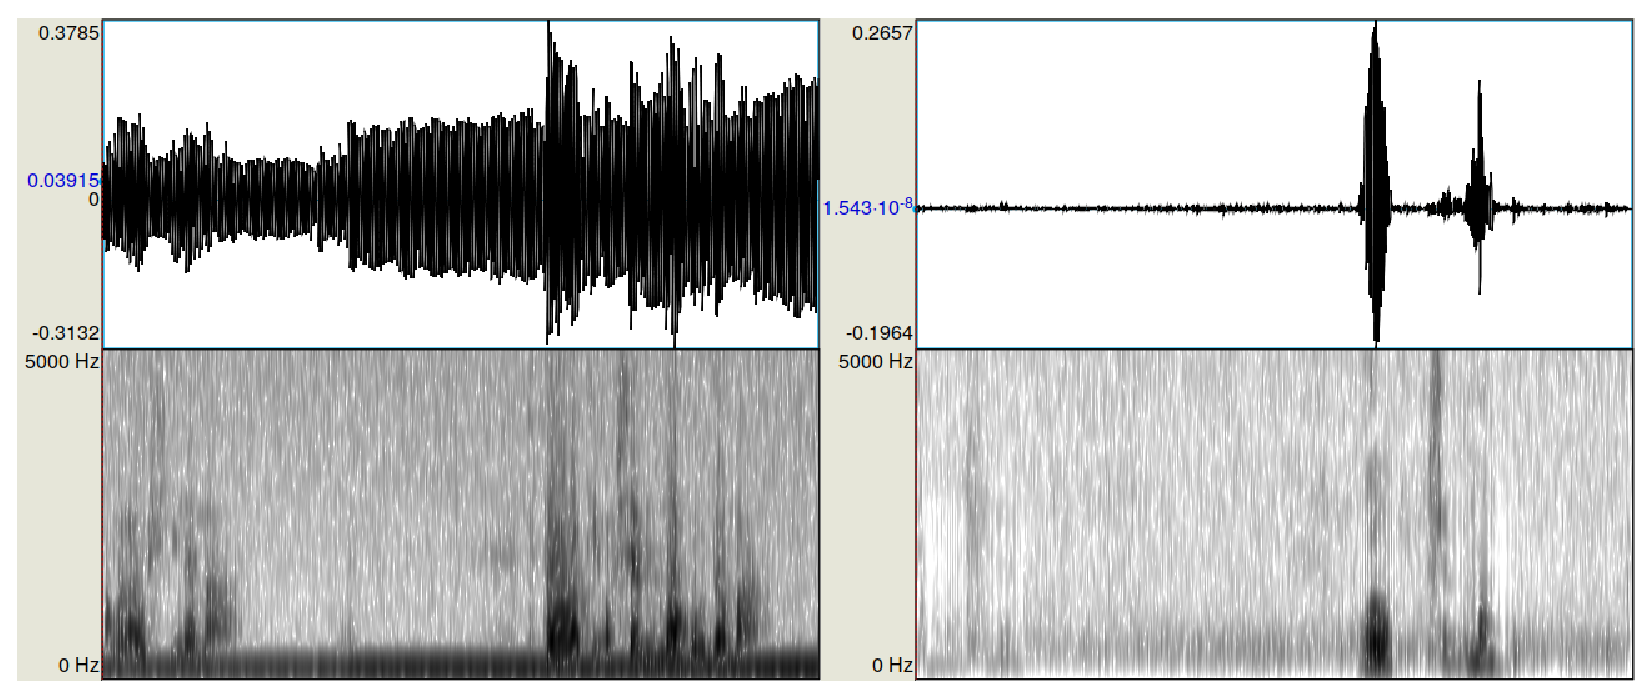
\includegraphics[scale=0.4]{rc/plzen.eps}
\caption{Wave form (above) and spectrogram (below) of a recording taken in low
tape speed before the CycleGAN transfer (left) and afterwards (right).}
\label{fig:plzen}
\end{figure}

\begin{figure}[htpb]
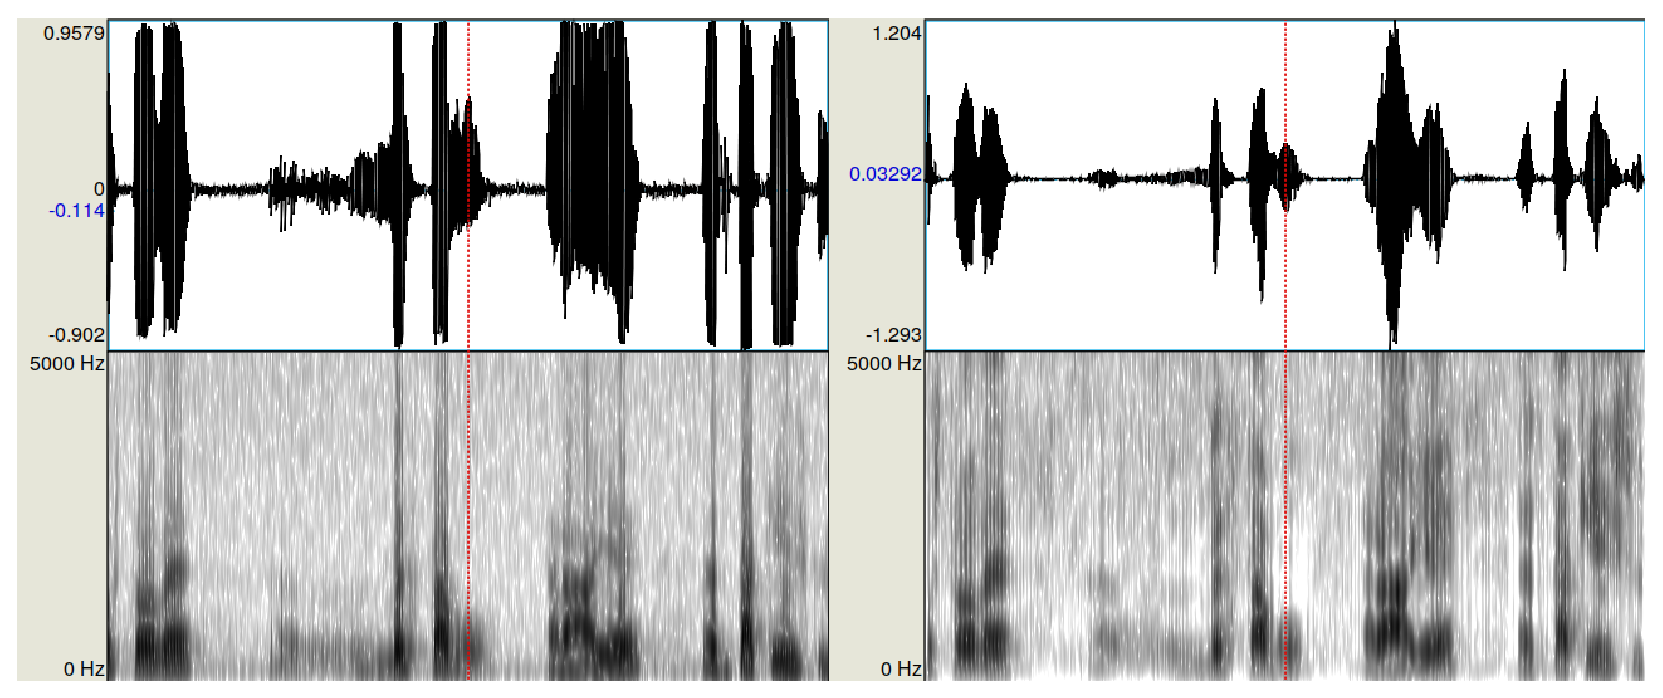
\includegraphics[scale=0.4]{rc/overdrive.eps}
\caption{Wave form (above) and spectrogram (below) of an overdriven recording
before the CycleGAN transfer (left) and afterwards (right).}
\label{fig:overdrive}
\end{figure}

%\subsection{Adapting CycleGAN for scattered domain}
%
%The way CycleGAN works given two datasets, one representing a domain $A$, the
%other representing a domain $B$, it learns two functions $f(A) -> B$ and
%$g(B) -> A$ that map the data between the two domains. In my case, where domain
%$B$ is not really a domain but more like a linear combination of several
%domains, the function $f$ that maps clean data to damaged data is not well
%defined. Indeed, how can we define a function that maps a clean recording to a
%damaged one when ``damaged'' can mean anything from overdrive, reverberation,
%noise, a frequency filter, and a number of other phenomena, and their
%combinations?
%
%A way could be to leverage the knowledge of the partially above listed possible
%effects that can turn a clean recording to a damaged one. If we defined
%elementary transformations simulating the individual ways a recording can be
%damaged, we could be looking for a linear combination of these transformations
%such that applying them on the clean sample $a \in A$ yields a result as similar
%to the damaged sample $b \in B$ as possible.
%
%Like this, we could make instead of $f(a \in A) -> B$ a function
%$f(a \in A, b \in B) -> B$ without the danger that it would degenerate to just
%returning the sample $b$.
%
%Aside of a metric for similarity between two sound files, we would need the list
%of transformations that take a substantial part in the acoustic damaging at
%hand.
%

\section{Conclusion}

Neural-network domain transfer offers a universally applicable method to
mitigate any kind and combination of acoustic defects without the necessity
of specifically modeling them. However,
we have not recorded any significant increase in speech recognition performance.
Also, where the damage is too severe, the processing discards the only
information at hand instead of improving its quality.

The benefit for human listeners seems quite promising although a quantitative
evaluation would be needed to assess it properly.

The conducted experiments on mitigating defects in acoustic quality of recorded speech
show that 1) it is not easy to reach an increase in speech recognition
performance, 2) it is easier to reach an improvement for the subjective
human listening experience and 3) heavily impaired recordings are particularly difficult to
make any better.

\section*{Acknowledgments}

This work has been supported by undisclosed institutions and entities.



\bibliographystyle{splncs}

\bibliography{citace}

\end{document}
